
%\graphicspath{{C:/Users/Akhil Jain/Desktop/Pics/}}

%\begin{center}
%\LARGE{\textbf{  Installation of Microsoft's Kinect for Windows SDK}}
%\end{center}


\begin{flushleft}

\chapter{Installation of necessary software}


\medskip
\section{\textbf{Installation of Kinect for Windows SDK (Windows)}}
\medskip
Hello world ! This is a quick installation tutorial for the Microsoft's Kinect for Windows SDK.
The Kinect for Windows Software Development Kit (SDK) enables developers to create applications that support gestures and voice recognition, using kinect sensor technology. Refer to \cite{download_sdk}.

\medskip
\textbf{Note : }
At the time of making of this manual, the latest version was Kinect for windows v.1.8.0 The same was used for experimenting with kinect.

\subsection{\textbf{ System Requirements}}
\medskip

\medskip
\begin{itemize}
\item Hardware Requirements
\medskip
\begin{itemize}
\item 32-bit (x86) or 64-bit (x64) processor
\item Dual-core 2.66-GHz or faster processor
\item Dedicated USB 2.0 bus
\item 2 GB RAM
\item A Microsoft Kinect for Windows (or Xbox) sensor
\end{itemize}
\medskip

\medskip
\item Software Requirements
\begin{itemize}
\item Visual Studio 2010, or Visual Studio 2012. The free Express editions can be downloaded from Microsoft Visual Studio 2010 Express or Microsoft Visual Studio 2012 Express.
\item .NET Framework 4 (installed with Visual Studio 2010), or .NET Framwork 4.5 (installed with Visual Studio 2012)
\item To develop speech-enabled Kinect for Windows Applications, you must install the Microsoft Speech Platform SDK v11
\medskip
\end{itemize}
\end{itemize}
\subsection{\textbf{ Installation Procedure}}
\addcontentsline{lof}{figure}{\textbf{Installation Procedure on Windows}}

\textbf{Step 1 :}

\medskip
1a) First the Microsoft's Kinect for windows SDK has to be downloaded. Download the same.
1b) Double click on the \textbf{KinectSDK-v1.8-Setup.exe} from the download location to begin the installation.  
Visit \url{ http://www.microsoft.com/en-in/download/details.aspx?id=40278.}

Shown in Figures \ref{fig:w1} and \ref{fig:w2} respectively.

\medskip
\textbf{Step 2 :}

\medskip
Accept the terms and conditions and click install.
Shown in Figure \ref{fig:w3}.

\medskip

\textbf{Step 3 :}

\medskip
The installation procedure will complete on its own.
Shown in Figure \ref{fig:w4}.

\medskip

\textbf{Step 4 :}

\medskip

After the installation of the SDK, download the Microsoft's Kinect for windows toolkit from the link in the window.
Shown in Figure \ref{fig:w5}.

\medskip

\textbf{Step 5 :}

\medskip

Double click on the \textbf{KinectDeveloperToolkit-v1.8.0-Setup.exe} from the download location to begin the installation. Accept the terms and conditions and click install.
Shown in Figure \ref{fig:w6}.
 
\medskip

\textbf{Step 6 :}

\medskip

The installation procedure will complete on its own.
Shown in Figure \ref{fig:w7}.

\medskip

\textbf{Step 7 :}

\medskip

Wait for the installation to complete.
Shown in Figure \ref{fig:w8}.

\medskip

\textbf{Step 8 :}

\medskip
Verify the installation by opening the Developer Toolkit Browser v.1.8.0
Shown in Figure \ref{fig:w9}.

\medskip

\medskip
\begin{figure}
\begin{center}
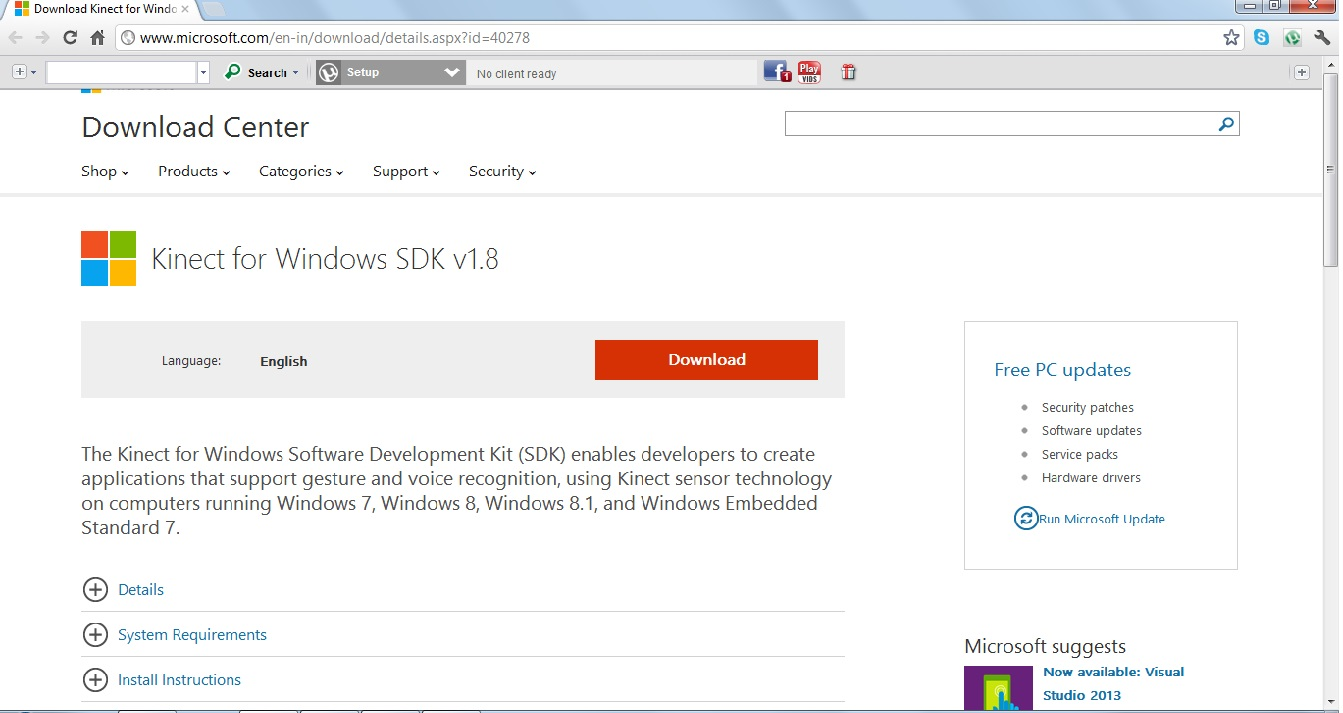
\includegraphics[scale=0.4]{website}
\end{center}
\caption{Step 1a - Microsoft's Kinect for Windows SDK website}
\label{fig:w1}
\end{figure}

\medskip
\begin{figure}
\begin{center}
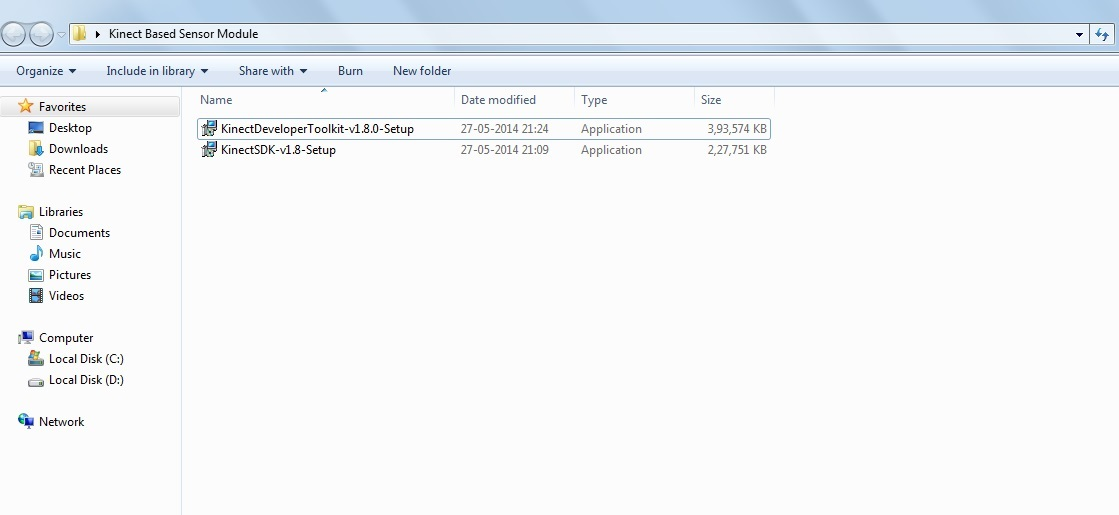
\includegraphics[scale=0.5]{downloaded}
\end{center}
\caption{Step 1b - The downloaded setup files}
\label{fig:w2}
\end{figure}
\medskip

\begin{figure}
\begin{center}
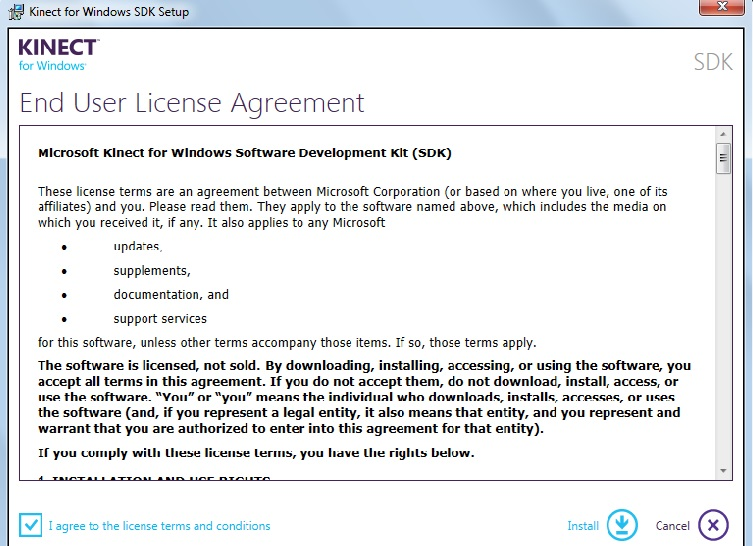
\includegraphics[scale=0.7]{sdk_step1}
\end{center}
\caption{Step 2 - Kinect for windows SDK setup}
\label{fig:w3}
\end{figure}

\medskip
\begin{figure}
\begin{center}
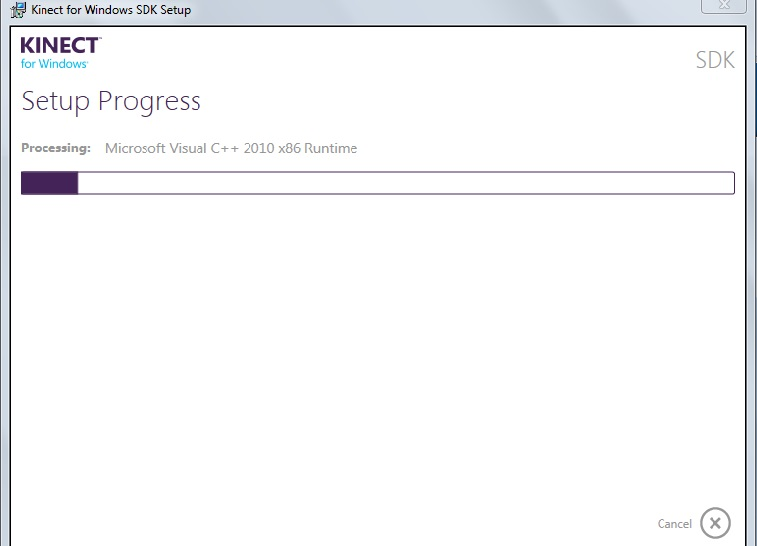
\includegraphics[scale=0.7]{sdk_step2}
\end{center}
\caption{Step 3 - Setup process will complete on its own}
\label{fig:w4}
\end{figure}
\medskip
\begin{figure}
\begin{center}
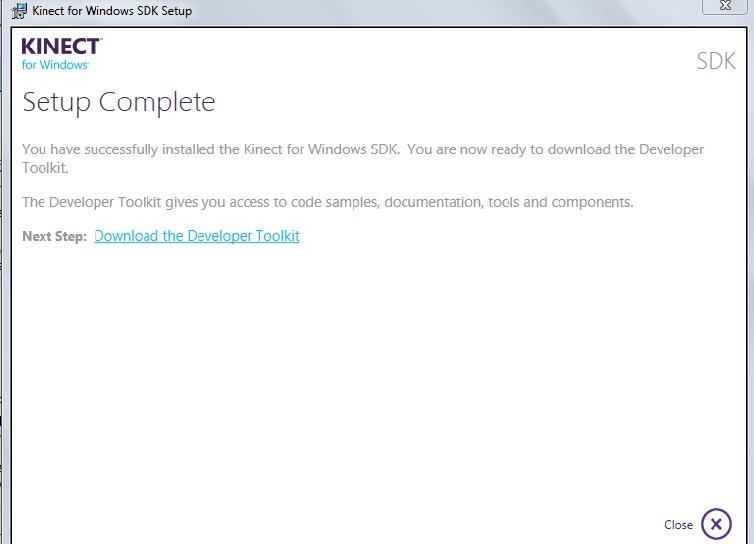
\includegraphics[scale=0.7]{sdk_step3}
\end{center}
\caption{Step 4 - Click on "Download the developer toolkit"}
\label{fig:w5}
\end{figure}

\medskip
\begin{figure}
\begin{center}
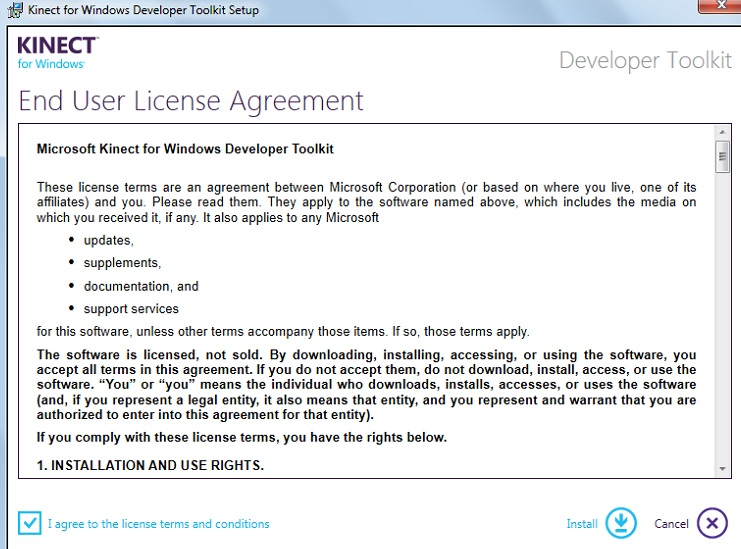
\includegraphics[scale=0.7]{toolkit_step1}
\end{center}
\caption{Step 5 - Kinect for Windows Developer toolkit setup}
\label{fig:w6}
\end{figure}
\medskip
\begin{figure}
\begin{center}
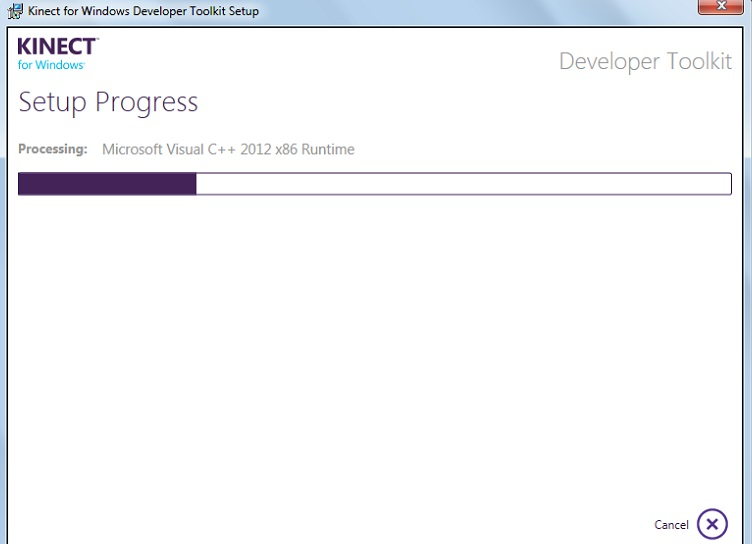
\includegraphics[scale=0.7]{toolkit_step2}
\end{center}
\caption{Step 6 - The toolkit setup will complete on its own}
\label{fig:w7}
\end{figure}

\medskip
\begin{figure}
\begin{center}
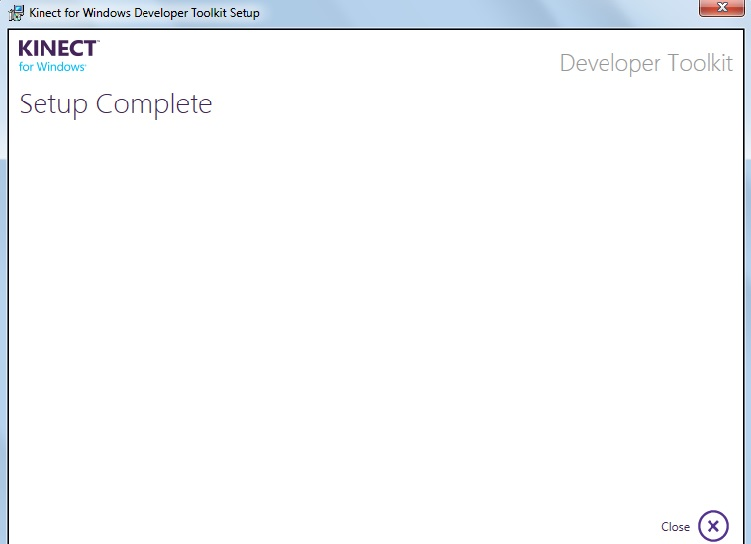
\includegraphics[scale=0.7]{toolkit_step3}
\end{center}
\caption{Step 7 - The setup is complete}
\label{fig:w8}
\end{figure}

\medskip
\begin{figure}
\begin{center}
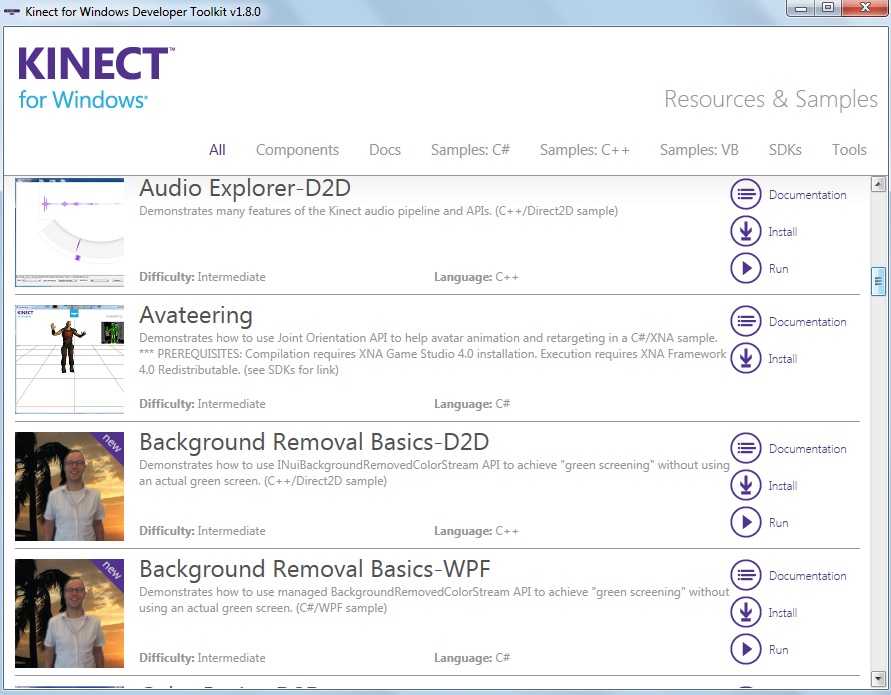
\includegraphics[scale=0.7]{after_install}
\end{center}
\caption{Step 8 - Kinect for windows Developer Toolkit v1.8.0}
\label{fig:w9}
\end{figure}

\medskip
\section{\textbf{Installation of Openkinect's Libfreenect (Ubuntu)}}
\medskip
Hello world ! This is a quick installation tutorial for the Openkinect's Libfreenect on the Linux platform. Ubuntu 14.04 is the platform used in this tutorial. Refer to \cite{openkinect}.


\subsection{\textbf{ System Requirements}}

\begin{itemize}
\item Hardware Requirements
\medskip
\begin{itemize}
\item 32-bit (x86) or 64-bit (x64) processor
\item Dual-core 2.66-GHz or faster processor
\item Dedicated USB 2.0 bus
\item 2 GB RAM
\item A Microsoft Kinect for Windows (or Xbox) sensor
\end{itemize}
\end{itemize}

\medskip

\subsection{\textbf{ Installation Procedure}}
\addcontentsline{lof}{figure}{\textbf{Installation Procedure on Ubuntu}}

\textbf{Step 1 :}

\medskip
Open a new terminal and type - 


\medskip

\framebox{\parbox{\dimexpr\linewidth-2\fboxsep-2\fboxrule}{sudo apt-get install git-core cmake libglut3-dev pkg-config build-essential libxmu-dev libxi-dev libusb-1.0-0-dev}}
\medskip

Enter the password when prompted. The installation will complete on its own.
\medskip

Note: If you getting an error saying apt-get cannot find libglut3, you might be on a newer version of Ubuntu that has freeglut3-* instead of libglut3-*, so your initial apt-get install would look like: 
\medskip

\framebox{\parbox{\dimexpr\linewidth-2\fboxsep-2\fboxrule}{sudo apt-get install git-core cmake freeglut3-dev pkg-config build-essential libxmu-dev libxi-dev libusb-1.0-0-devgit}}

\medskip
Shown in Figure \ref{fig:w10}.
\medskip

\textbf{Step 2 :}

\medskip

Clone the Libfreenect file from Github base by typing 

\medskip

\framebox{\parbox{\dimexpr\linewidth-2\fboxsep-2\fboxrule}{clone git://github.com/OpenKinect/libfreenect.git}}

\medskip

At the completion of cloning you will find a folder named \textbf{libfreenect} in your home directory.

\medskip
Shown in Figure \ref{fig:w11}.

\medskip
\textbf{Step 3 :}

\medskip

Enter the libfreenect folder by typing - 

\medskip

\framebox{\parbox{\dimexpr\linewidth-2\fboxsep-2\fboxrule}{cd libfreenect}}

\medskip
Shown in Figure \ref{fig:w12}.

\medskip
\textbf{Step 4 :}

\medskip

Make a new directory in the libfreenect folder and name it 'build'

\medskip

\framebox{\parbox{\dimexpr\linewidth-2\fboxsep-2\fboxrule}{mkdir build}}

\medskip
Shown in Figure \ref{fig:w13}.

\medskip
\textbf{Step 5 :}

\medskip

Enter the build directory by typing - 

\medskip

\framebox{\parbox{\dimexpr\linewidth-2\fboxsep-2\fboxrule}{cd build}}

\medskip
Shown in Figure \ref{fig:w14}.

\medskip

\textbf{Step 6 :}

\medskip

6a) Now "make" all the projects by typing - 

\medskip

\framebox{\parbox{\dimexpr\linewidth-2\fboxsep-2\fboxrule}{cmake ..}}

\medskip 

6b) and then type

\medskip

\framebox{\parbox{\dimexpr\linewidth-2\fboxsep-2\fboxrule}{make}}

\medskip
Shown in Figures \ref{fig:w15} and \ref{fig:w16} respectively

\medskip
\textbf{Step 7 :}

\medskip

Next Type - 

\medskip

\framebox{\parbox{\dimexpr\linewidth-2\fboxsep-2\fboxrule}{sudo make install}}

\medskip
Shown in Figure \ref{fig:w17}.

\medskip
\textbf{Step 8 :}

\medskip

Configure all the libraries by typing - 

\medskip

\framebox{\parbox{\dimexpr\linewidth-2\fboxsep-2\fboxrule}{sudo ldconfig /usr/local/lib64/}}

\medskip

Shown in Figure \ref{fig:w18}.

\medskip
\textbf{Step 9 :}

\medskip

To use Kinect as a non-root user type the following -

\medskip

\framebox{\parbox{\dimexpr\linewidth-2\fboxsep-2\fboxrule}{sudo adduser \$USER video}}

\medskip
Shown in Figure \ref{fig:w19}.

\medskip

\medskip

\textbf{Step 10 :}

\medskip

Now for testing the installed software we will run one of the sample projects by typing - 

\medskip

\framebox{\parbox{\dimexpr\linewidth-2\fboxsep-2\fboxrule}{sudo freenect-glview}}

\medskip

Shown in Figure \ref{fig:w20}.
\medskip

The Ouput is shown in Figure \ref{fig:w21}.

\medskip

\textbf{Note :}

\begin{itemize}
\item The installation procedure for other platforms is available on 
 \medskip
 
 \url{http://openkinect.org/wiki/Getting\_Started}

\item One can also make a file with rules for the Linux device manager:
 
 \framebox{\parbox{\dimexpr\linewidth-2\fboxsep-2\fboxrule}{sudo nano /etc/udev/rules.d/51-kinect.rules}}
 
 Copy and paste:
 
 
 \framebox{\parbox{\dimexpr\linewidth-2\fboxsep-2\fboxrule}{
 \# ATTR{product}=="Xbox NUI Motor"
 SUBSYSTEM=="usb",
  ATTR{idVendor}=="045e", ATTR{idProduct}=="02b0", MODE="0666"
  
 \# ATTR{product}=="Xbox NUI Audio"
 SUBSYSTEM=="usb",
  ATTR{idVendor}=="045e", ATTR{idProduct}=="02ad", MODE="0666"
  
 \# ATTR{product}=="Xbox NUI Camera"
 SUBSYSTEM=="usb",
  ATTR{idVendor}=="045e", ATTR{idProduct}=="02ae", MODE="0666"
  
 \# ATTR{product}=="Xbox NUI Motor"
 SUBSYSTEM=="usb",
  ATTR{idVendor}=="045e", ATTR{idProduct}=="02c2", MODE="0666"
  
 \# ATTR{product}=="Xbox NUI Motor"
 SUBSYSTEM=="usb",
  ATTR{idVendor}=="045e", ATTR{idProduct}=="02be", MODE="0666"
  
 \# ATTR{product}=="Xbox NUI Motor"
 SUBSYSTEM=="usb",
  ATTR{idVendor}=="045e", ATTR{idProduct}=="02bf", MODE="0666"
  
  }}
 \medskip
 
 Be sure to log out and back in. 
 
\end{itemize}
\begin{figure}
\begin{center}
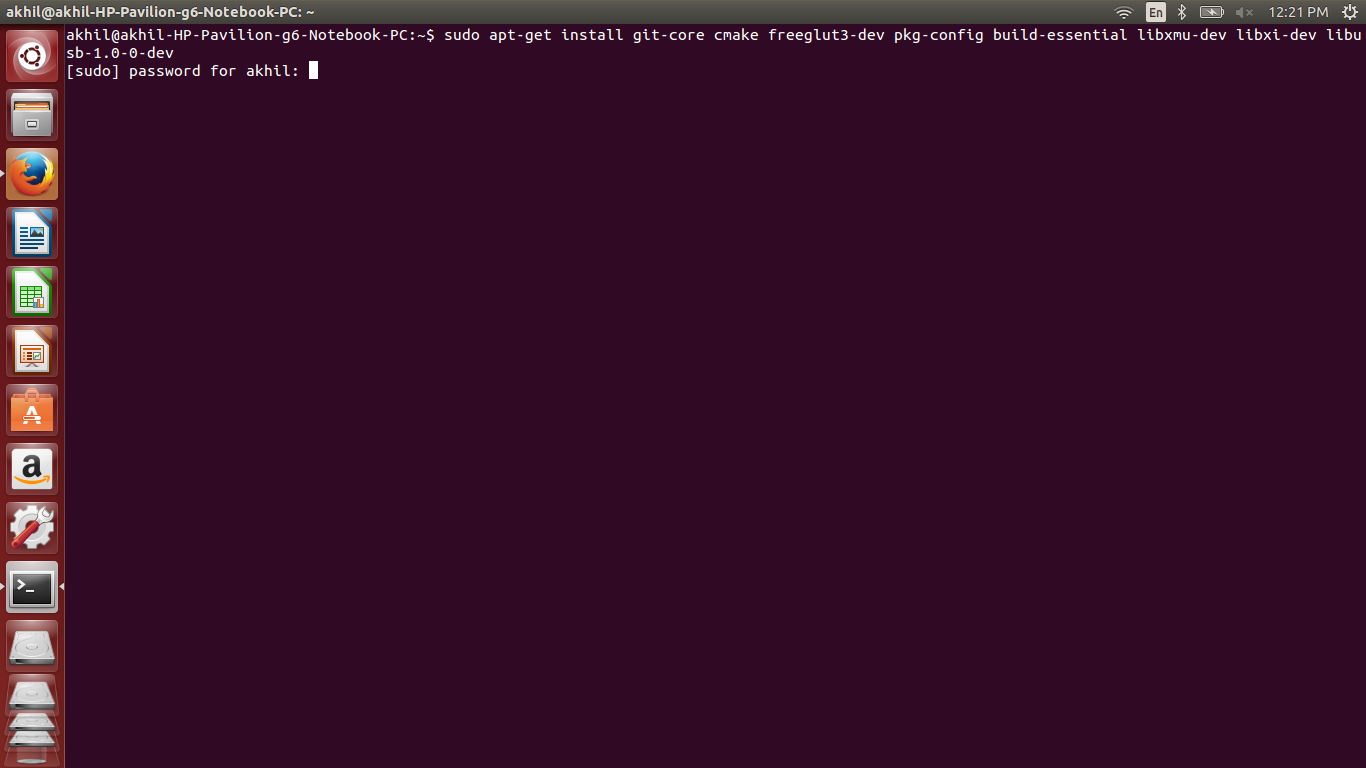
\includegraphics[scale=0.35]{step1}
\end{center}
\caption{Step 1 - Installation}
\label{fig:w10}
\end{figure}
\medskip
\begin{figure}
\begin{center}
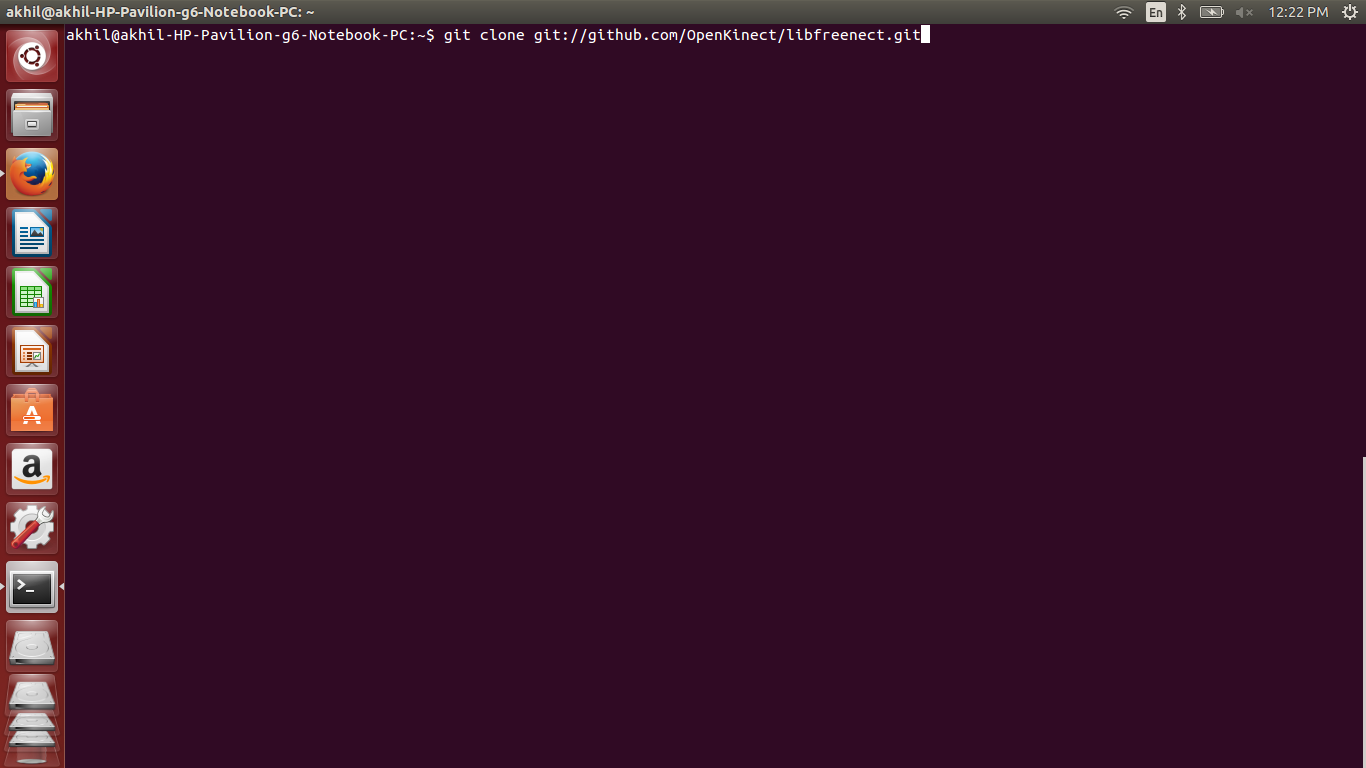
\includegraphics[scale=0.35]{step2}
\end{center}
\caption{Step 2 - Cloning libfreenect}
\label{fig:w11}
\end{figure}
\medskip
\begin{figure}
\begin{center}
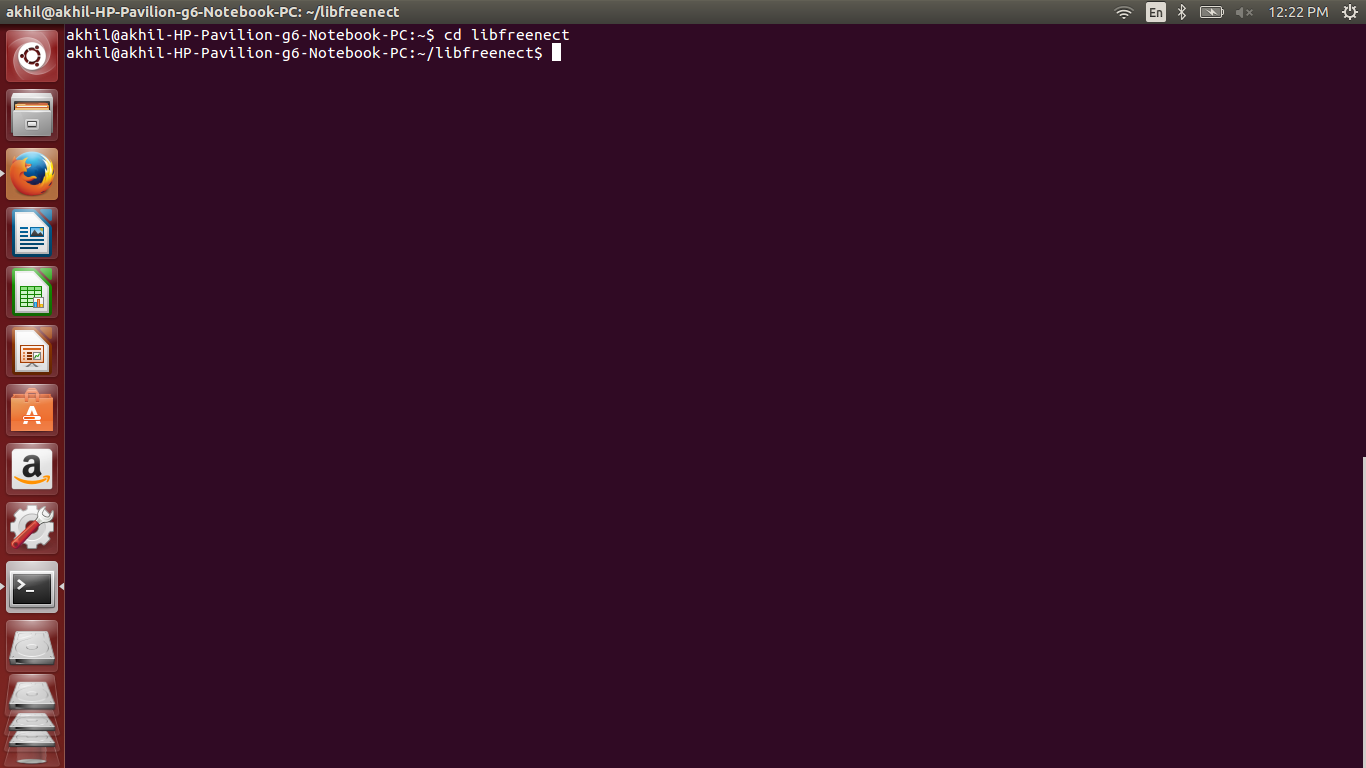
\includegraphics[scale=0.35]{step3}
\end{center}
\caption{Step 3 - Enter the libfreenect folder}
\label{fig:w12}
\end{figure}
\medskip
\begin{figure}
\begin{center}
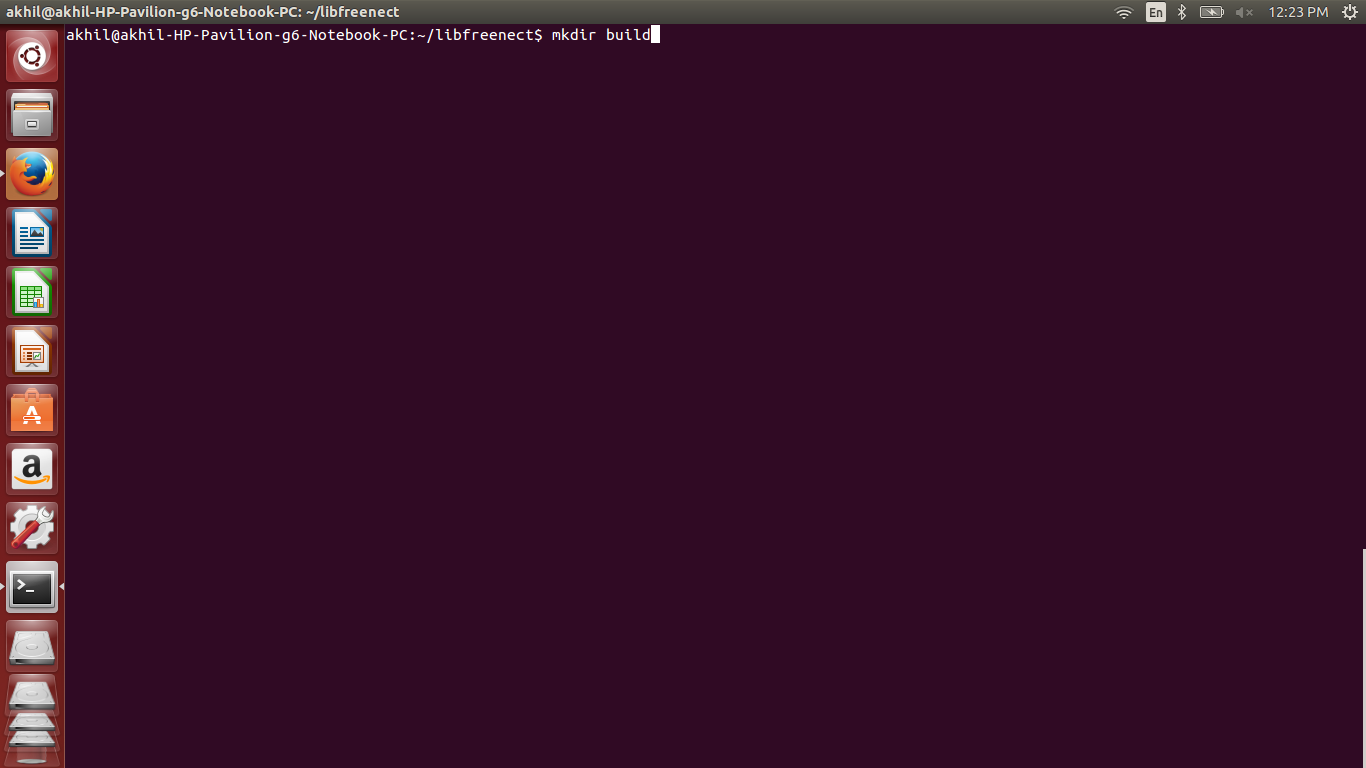
\includegraphics[scale=0.35]{step4}
\end{center}
\caption{Step 4 - Create a new directory named "build"}
\label{fig:w13}
\end{figure}
\medskip
\begin{figure}
\begin{center}
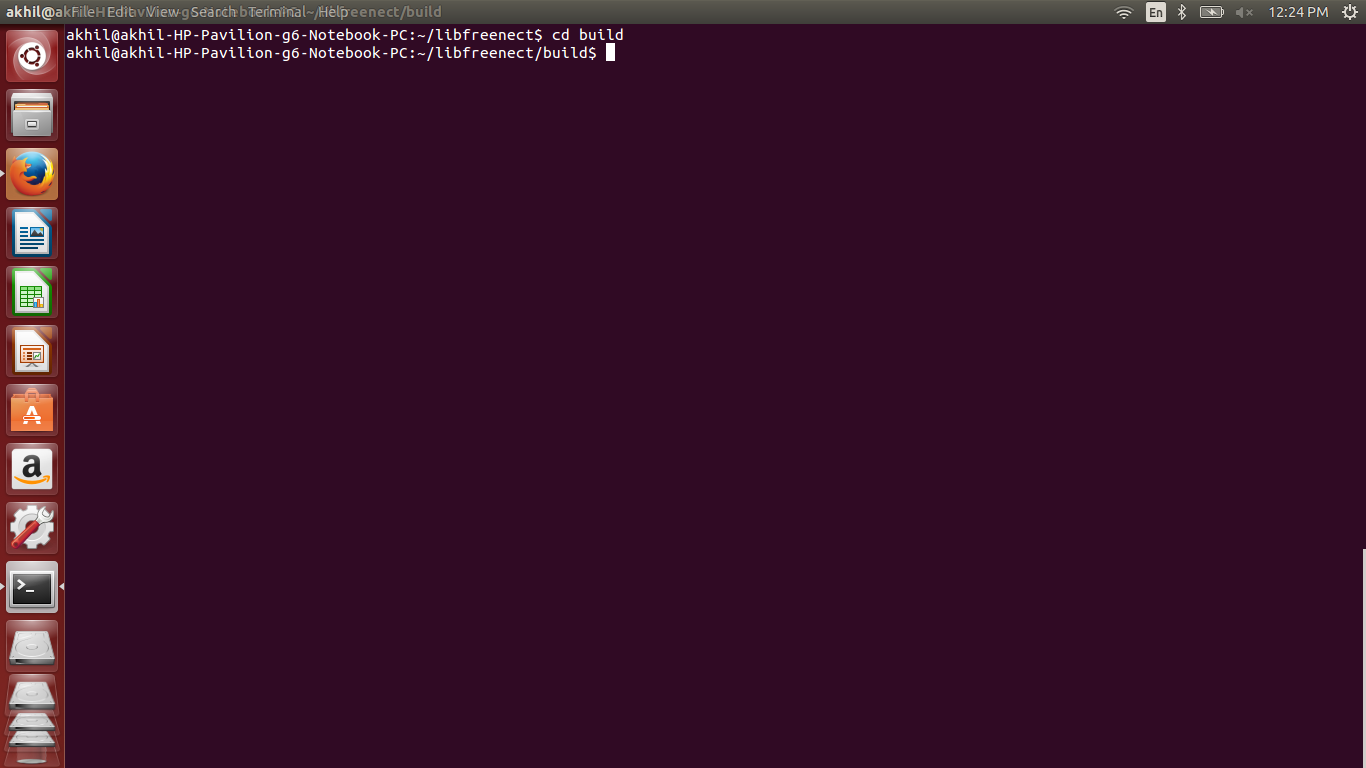
\includegraphics[scale=0.35]{step5}
\end{center}
\caption{Step 5 - Enter the build directory}
\label{fig:w14}
\end{figure}
\medskip
\begin{figure}
\begin{center}
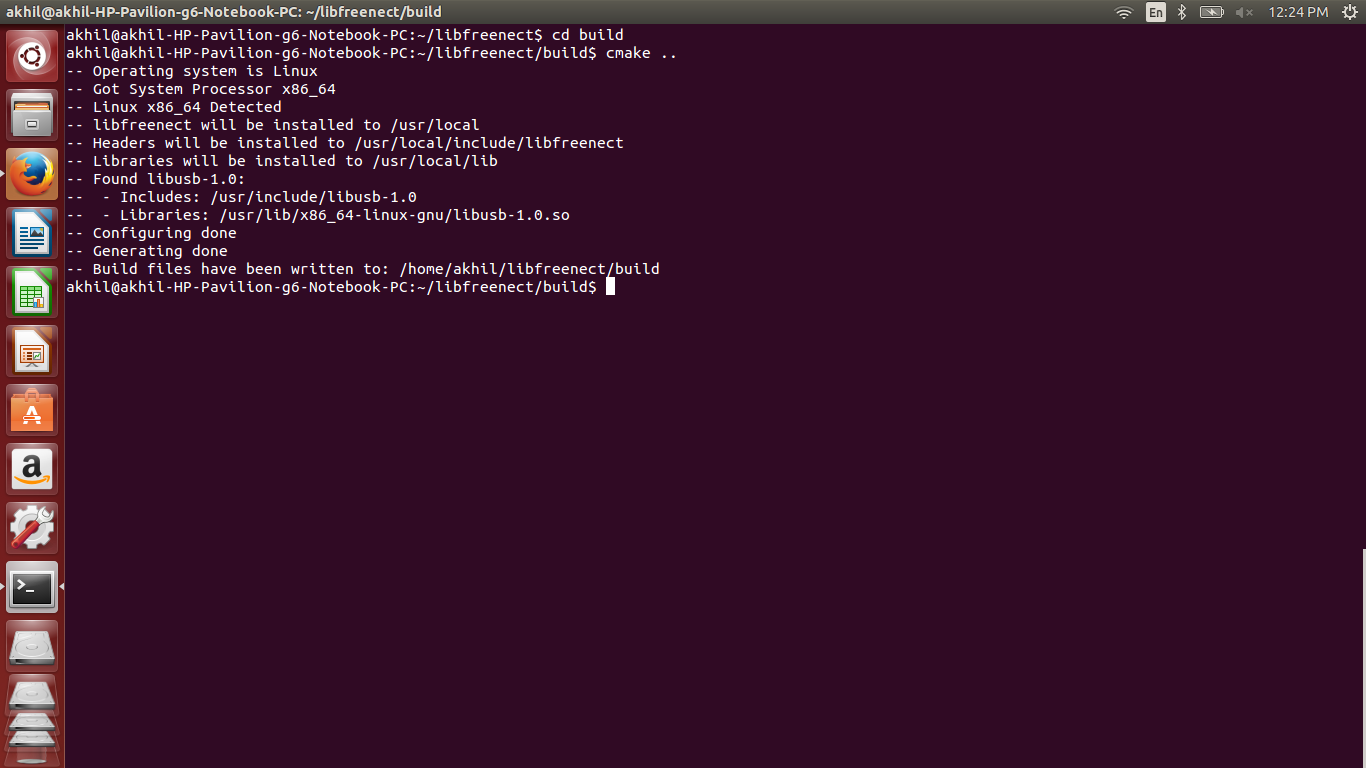
\includegraphics[scale=0.35]{step6}
\end{center}
\caption{Step 6a - cmake ..}
\label{fig:w15}
\end{figure}
\medskip
\begin{figure}
\begin{center}
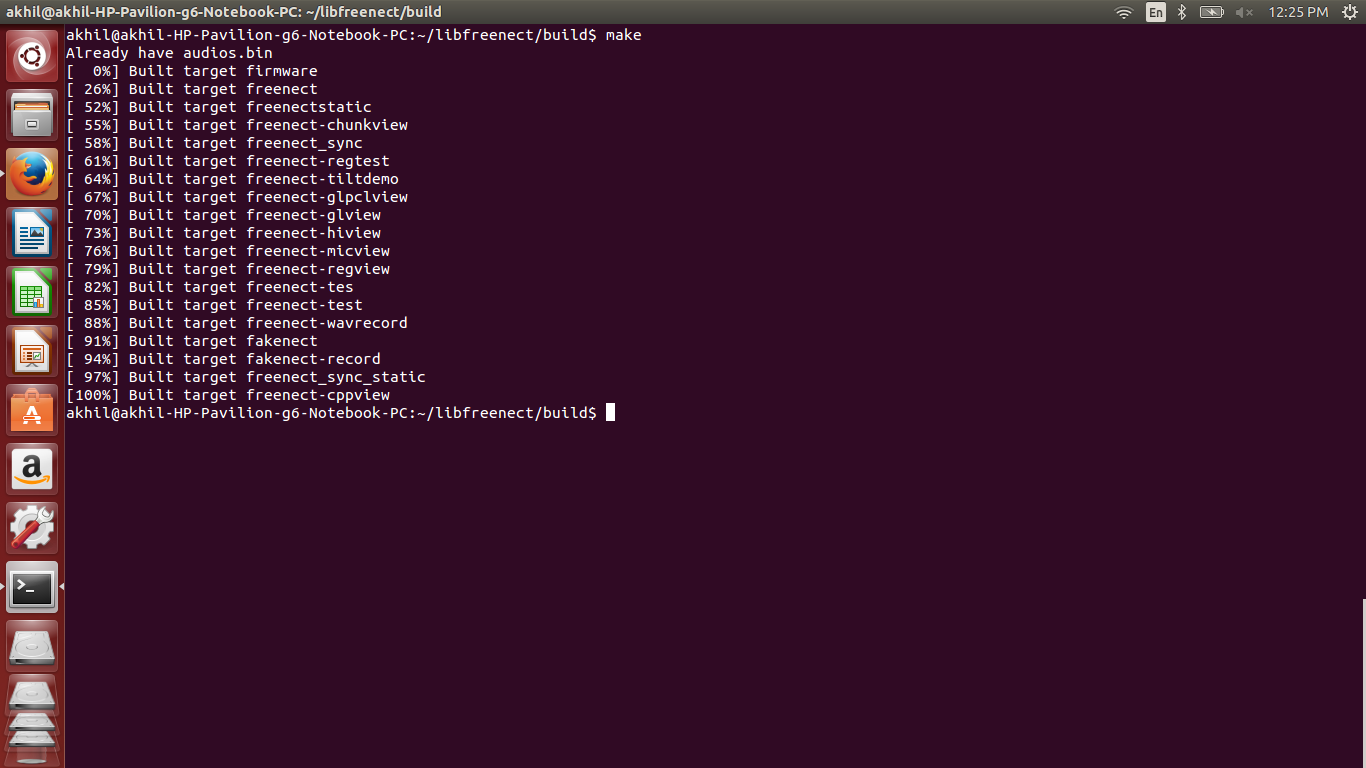
\includegraphics[scale=0.35]{step7}
\end{center}
\caption{Step 6b - make}
\label{fig:w16}
\end{figure}
\medskip
\begin{figure}
\begin{center}
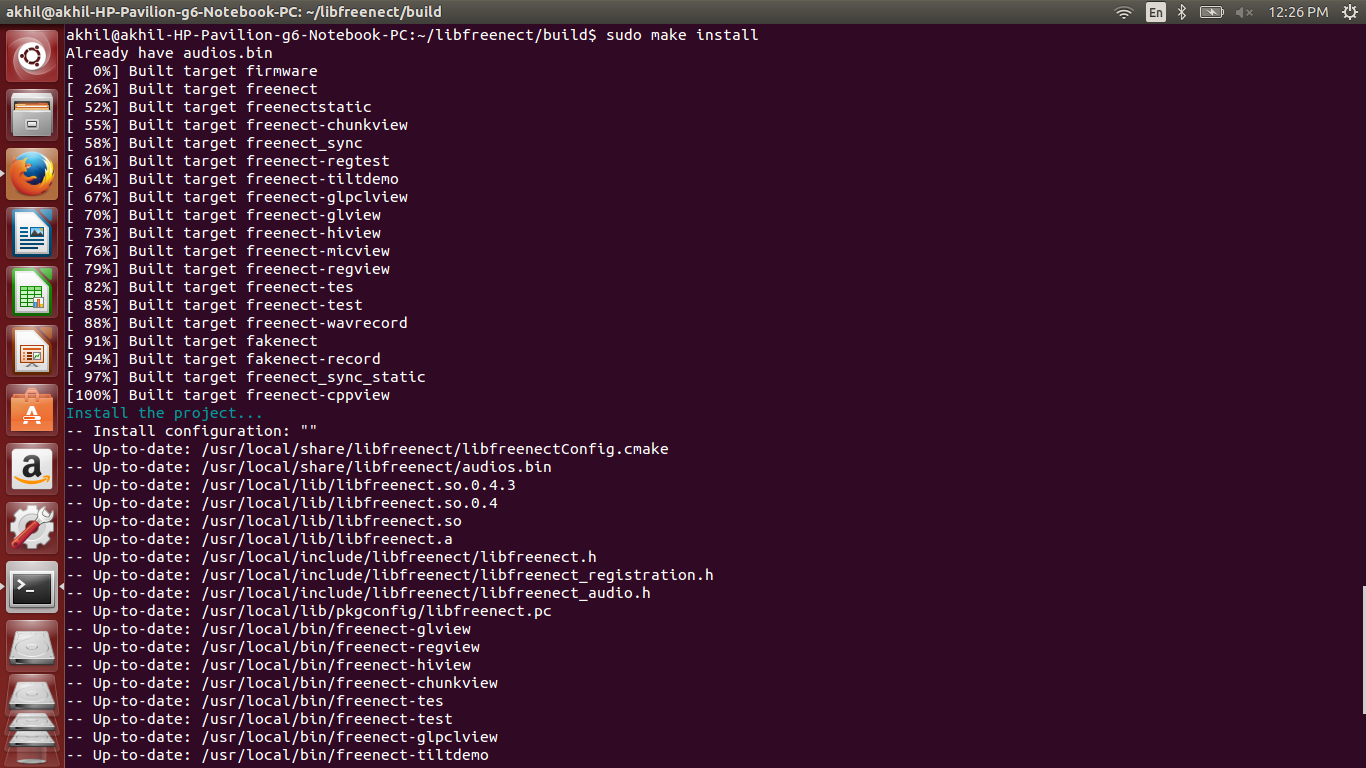
\includegraphics[scale=0.35]{step8}
\end{center}
\caption{Step 7 - sudo make install}
\label{fig:w17}
\end{figure}
\medskip
\begin{figure}
\begin{center}
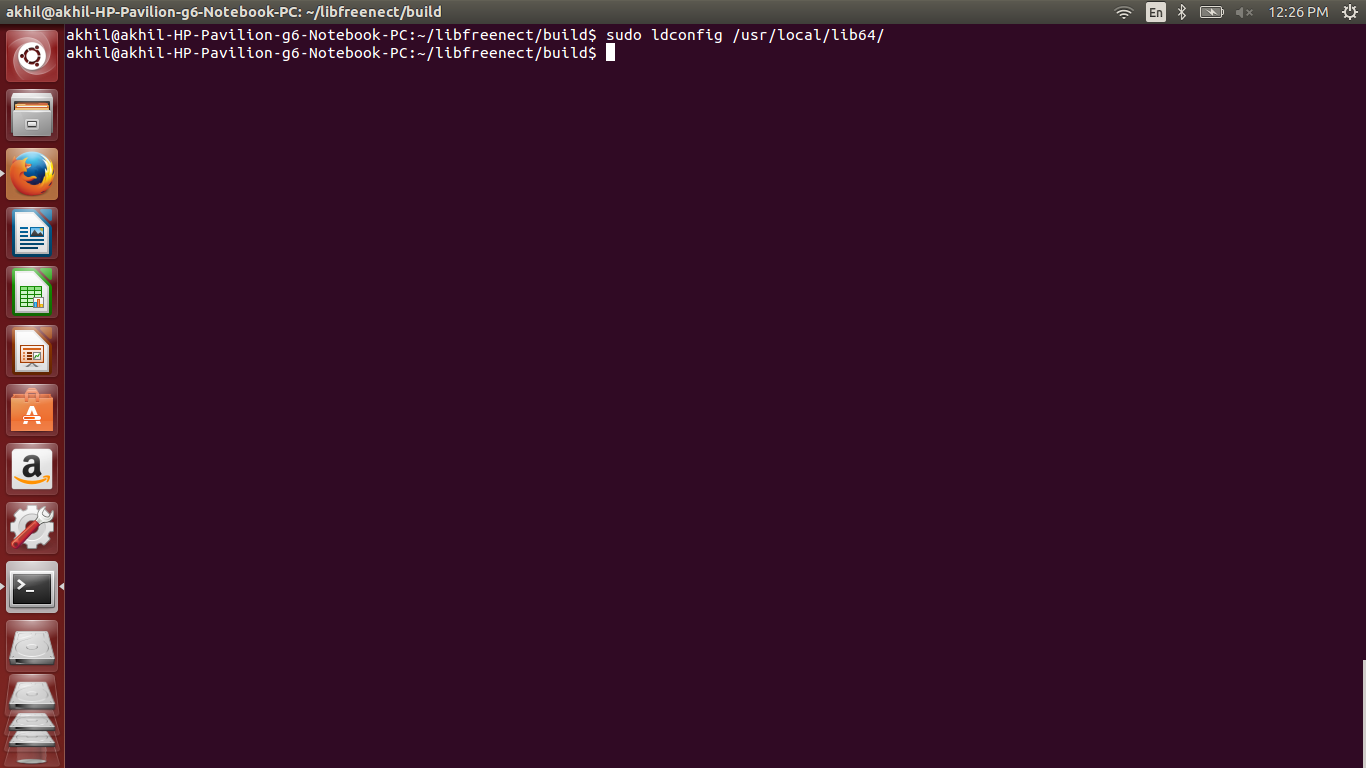
\includegraphics[scale=0.35]{step9}
\end{center}
\caption{Step 8 - Configuring the libraries}
\label{fig:w18}
\end{figure}
\medskip
\begin{figure}
\begin{center}
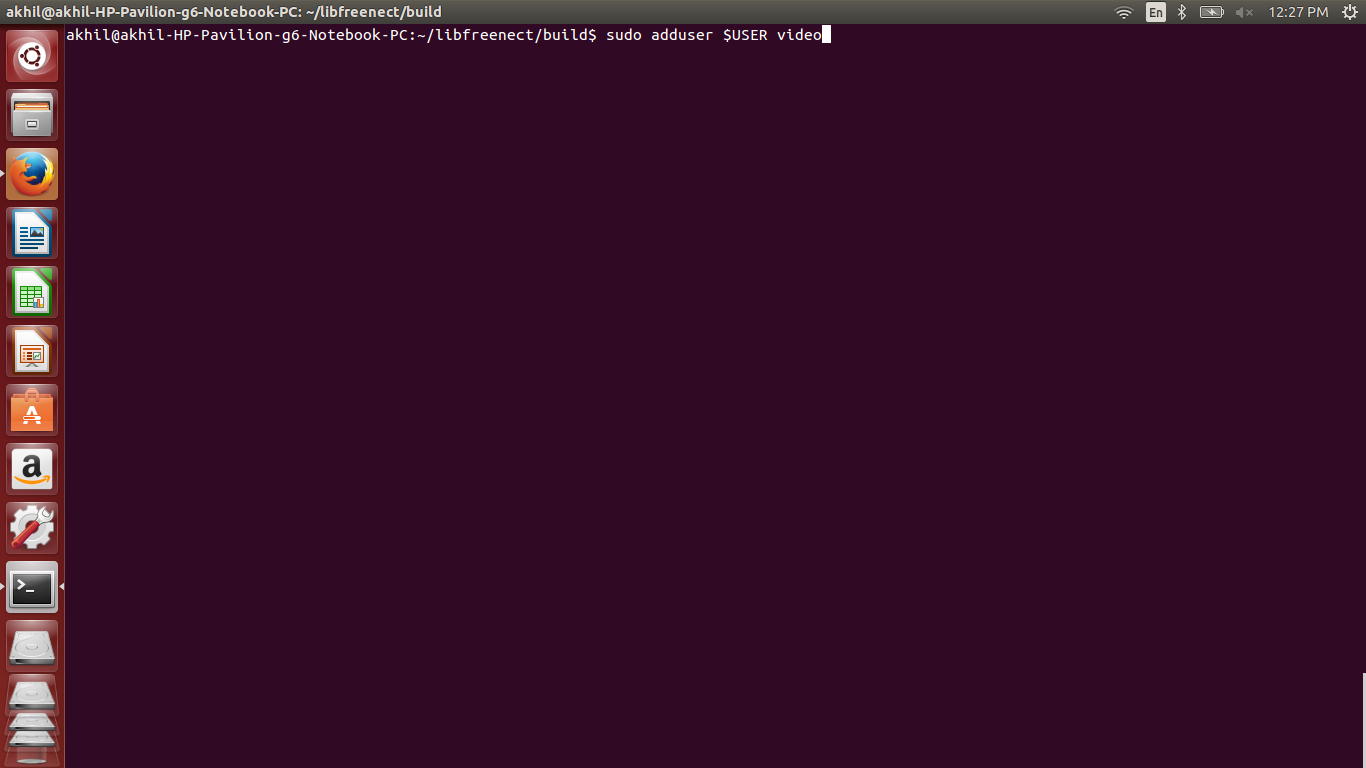
\includegraphics[scale=0.35]{step10}
\end{center}
\caption{Step 9 - To use kinect as a non-root user}
\label{fig:w19}
\end{figure}
\medskip
\begin{figure}
\begin{center}
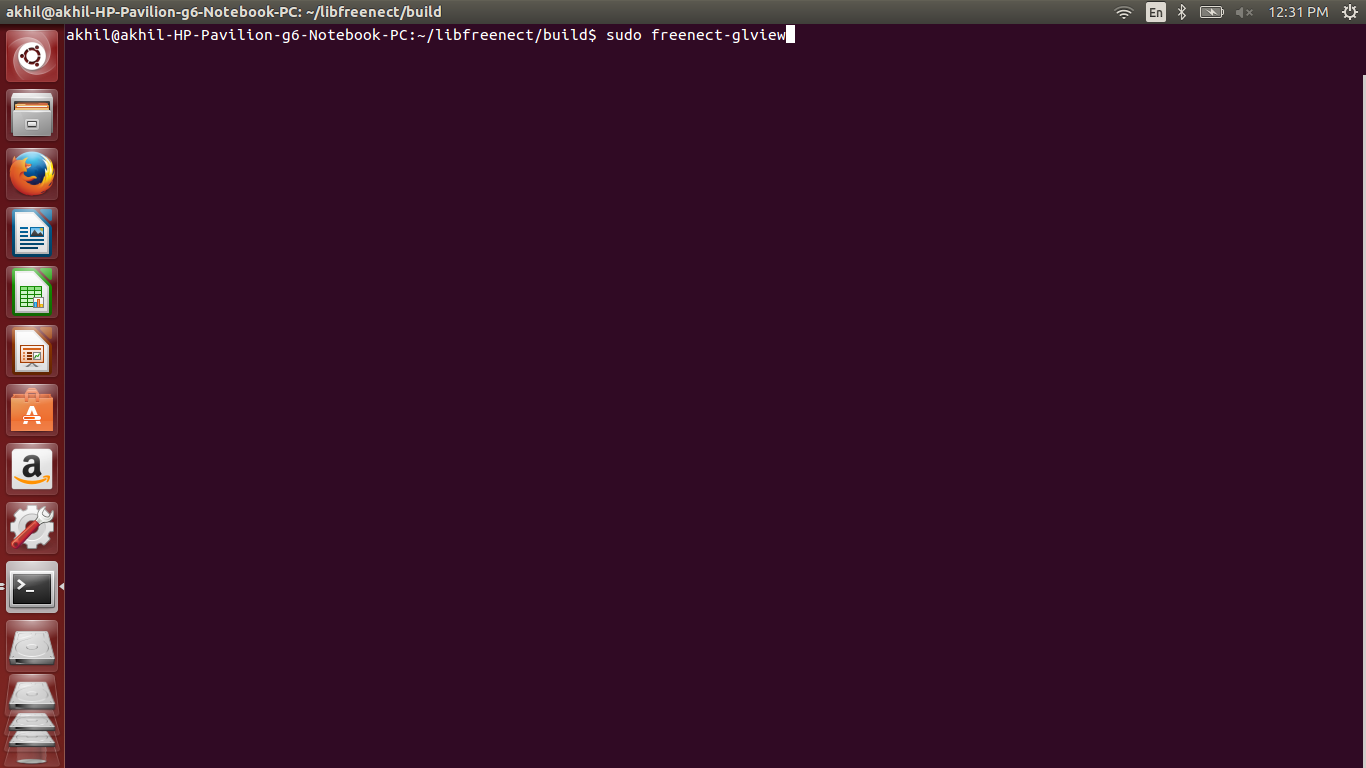
\includegraphics[scale=0.35]{step12}
\end{center}
\caption{Step 10 - Run a sample project}
\label{fig:w20}
\end{figure}
\medskip
\begin{figure}
\begin{center}
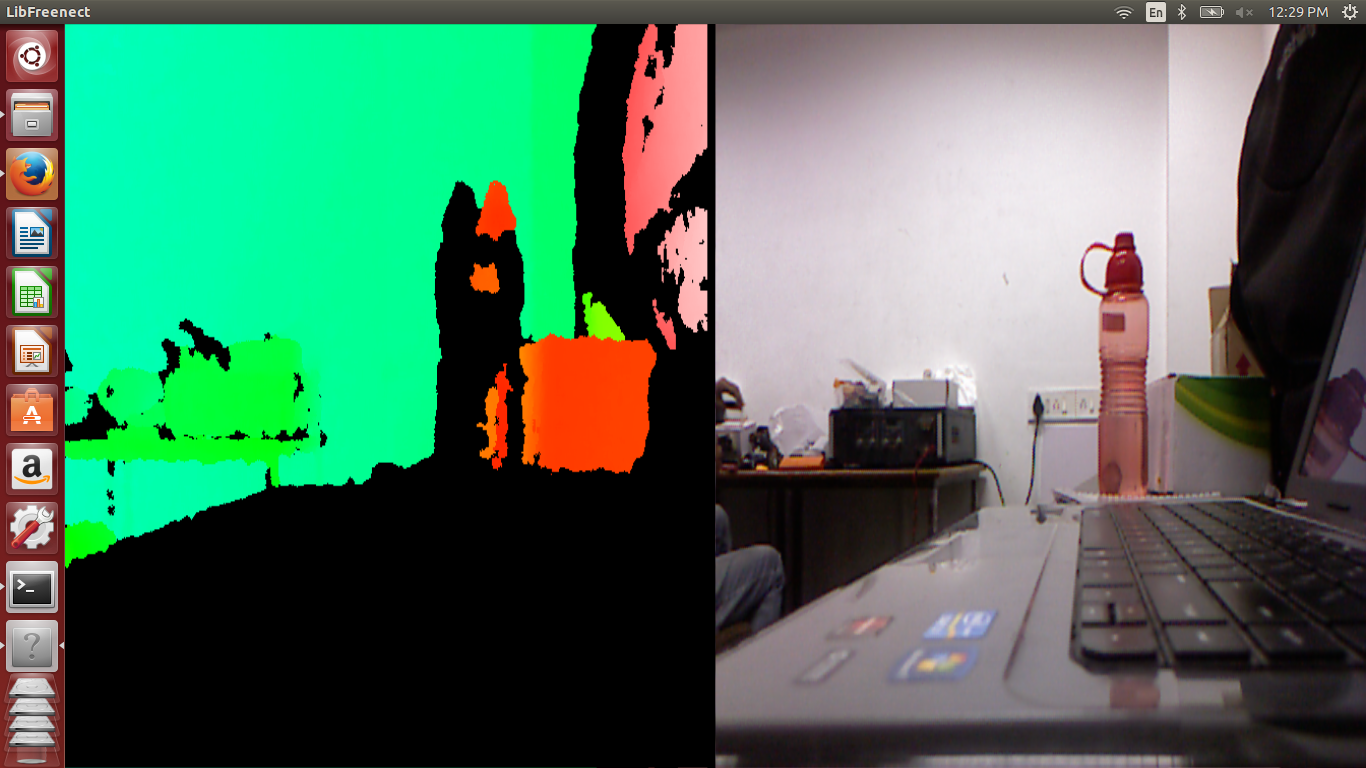
\includegraphics[scale=0.35]{step11}
\end{center}
\caption{Depth Image and Live Stream Video}
\label{fig:w21}
\end{figure}

\Large{\textbf{Congratulations ! You have just installed the necessary software for your platform to work on the Kinect sensor.}}


\end{flushleft}

